\documentclass{article}  
% Include all project wide packages here.
\usepackage{fullpage}
\usepackage{polyglossia}
\setmainlanguage{dutch}
\usepackage{csquotes}
\usepackage{graphicx}
\usepackage{epstopdf}
\usepackage{pdfpages}
\usepackage{caption}
\usepackage[list=true]{subcaption}
\usepackage{float}
%\usepackage{mathtools}
\usepackage{standalone}
\usepackage{import}
\usepackage{tocloft}
\usepackage{wrapfig}
\usepackage{authblk}
\usepackage{array}
\usepackage{booktabs}
\usepackage[toc,page,title,titletoc]{appendix}
\usepackage{xunicode}
\usepackage{amsmath}
\usepackage{fontspec}
\usepackage{unicode-math}
\usepackage[
    backend=bibtexu,
	texencoding=utf8,
bibencoding=utf8,
    style=ieee,
    sortlocale=nl_NL,
    language=auto
]{biblatex}
\usepackage{listings}
\newcommand{\includecode}[3][c]{\lstinputlisting[caption=#2, escapechar=, style=#1]{#3}}
\newcommand{\superscript}[1]{\ensuremath{^{\textrm{#1}}}}
\newcommand{\subscript}[1]{\ensuremath{_{\textrm{#1}}}}


\newcommand{\chapternumber}{\thechapter}
\renewcommand{\appendixname}{Bijlage}
\renewcommand{\appendixtocname}{Bijlagen}
\renewcommand{\appendixpagename}{Bijlagen}

\usepackage[hidelinks]{hyperref} %<--------ALTIJD ALS LAATSTE
  
\renewcommand{\familydefault}{\sfdefault}

\setmainfont[Ligatures=TeX]{Myriad Pro}
\setmathfont{Asana Math}
\setmonofont{Lucida Console}

\usepackage{titlesec, blindtext, color}
\definecolor{gray75}{gray}{0.75}
\newcommand{\hsp}{\hspace{20pt}}
\titleformat{\chapter}[hang]{\Huge\bfseries}{\chapternumber\hsp\textcolor{gray75}{|}\hsp}{0pt}{\Huge\bfseries}
\renewcommand{\familydefault}{\sfdefault}
\renewcommand{\arraystretch}{1.2}
\setlength\parindent{0pt}

%For code listings
\definecolor{black}{rgb}{0,0,0}
\definecolor{browntags}{rgb}{0.65,0.1,0.1}
\definecolor{bluestrings}{rgb}{0,0,1}
\definecolor{graycomments}{rgb}{0.4,0.4,0.4}
\definecolor{redkeywords}{rgb}{1,0,0}
\definecolor{bluekeywords}{rgb}{0.13,0.13,0.8}
\definecolor{greencomments}{rgb}{0,0.5,0}
\definecolor{redstrings}{rgb}{0.9,0,0}
\definecolor{purpleidentifiers}{rgb}{0.01,0,0.01}


\lstdefinestyle{csharp}{
language=[Sharp]C,
showspaces=false,
showtabs=false,
breaklines=true,
showstringspaces=false,
breakatwhitespace=true,
escapeinside={(*@}{@*)},
columns=fullflexible,
commentstyle=\color{greencomments},
keywordstyle=\color{bluekeywords}\bfseries,
stringstyle=\color{redstrings},
identifierstyle=\color{purpleidentifiers},
basicstyle=\ttfamily\small}

\lstdefinestyle{c}{
language=C,
showspaces=false,
showtabs=false,
breaklines=true,
showstringspaces=false,
breakatwhitespace=true,
escapeinside={(*@}{@*)},
columns=fullflexible,
commentstyle=\color{greencomments},
keywordstyle=\color{bluekeywords}\bfseries,
stringstyle=\color{bluestrings},
identifierstyle=\color{purpleidentifiers}
}

\lstdefinestyle{vhdl}{
language=VHDL,
showspaces=false,
showtabs=false,
breaklines=true,
showstringspaces=false,
breakatwhitespace=true,
escapeinside={(*@}{@*)},
columns=fullflexible,
commentstyle=\color{greencomments},
keywordstyle=\color{bluekeywords}\bfseries,
stringstyle=\color{redstrings},
identifierstyle=\color{purpleidentifiers}
}

\lstdefinestyle{xaml}{
language=XML,
showspaces=false,
showtabs=false,
breaklines=true,
showstringspaces=false,
breakatwhitespace=true,
escapeinside={(*@}{@*)},
columns=fullflexible,
commentstyle=\color{greencomments},
keywordstyle=\color{redkeywords},
stringstyle=\color{bluestrings},
tagstyle=\color{browntags},
morestring=[b]",
  morecomment=[s]{<?}{?>},
  morekeywords={xmlns,version,typex:AsyncRecords,x:Arguments,x:Boolean,x:Byte,x:Char,x:Class,x:ClassAttributes,x:ClassModifier,x:Code,x:ConnectionId,x:Decimal,x:Double,x:FactoryMethod,x:FieldModifier,x:Int16,x:Int32,x:Int64,x:Key,x:Members,x:Name,x:Object,x:Property,x:Shared,x:Single,x:String,x:Subclass,x:SynchronousMode,x:TimeSpan,x:TypeArguments,x:Uid,x:Uri,x:XData,Grid.Column,Grid.ColumnSpan,Click,ClipToBounds,Content,DropDownOpened,FontSize,Foreground,Header,Height,HorizontalAlignment,HorizontalContentAlignment,IsCancel,IsDefault,IsEnabled,IsSelected,Margin,MinHeight,MinWidth,Padding,SnapsToDevicePixels,Target,TextWrapping,Title,VerticalAlignment,VerticalContentAlignment,Width,WindowStartupLocation,Binding,Mode,OneWay,xmlns:x}
}

%defaults
\lstset{
basicstyle=\ttfamily\small,
extendedchars=false,
numbers=left,
numberstyle=\ttfamily\tiny,
stepnumber=1,
tabsize=4,
numbersep=5pt
} 
\addbibresource{../../library/bibliography.bib}

\author{Robin Hes (4236815) \and Jorden Kerkhof (3458923)}

\title{EPO3-1 - Opdracht 4: Unified Model Parameters}
\date{3 oktober 2013}
\begin{document}
\maketitle

\section{Abstract}
\label{sec:ump-abstr}

\tableofcontents

\section{Inleiding}
\label{sec:ump-inl}

\section{Probleemstelling}
\label{sec:ump-prob}

\section{Theorie}
\label{sec:ump-theorie}
In SPICE-simulaties wordt uiteraard een model gebruikt, dat een werkelijke transistor zo goed mogelijk nabootst. Een computer rekent immers veel sneller dan een mens en dus is de complexiteit van het model een minder groot probleem. Voor handmatige analyse van een CMOS-transistor is het echter wenselijk om een model te hebben dat ook voor de mens te gebruiken is.
Het unified transistormodel van Rabaey biedt hier een uitkomst. Het model beschrijft, met slechts een enkele vergelijking, de drainstroom $I_{D}$ door de transistor, aan de hand van een vrij beperkt aantal parameters. De drainstroom wordt gemodelleerd in de drie verschillende werkgebieden waarin de transistor zich kan bevinden, wanneer deze in geleiding is, afhankelijk van de spanning over drain en source ($V_{DS}$). Daarnaast beschrijft het model de effecten van velocity saturation.
De vergelijking voor $I_{D}$, zoals gegeven door Rabaey, is als volgt:

\begin{equation} \label{eq:ump-cmos-model-rab}
	I_{D} = k' \frac{W}{L} (V_{GT}V_{min} - \frac{V_{min}^2}{2})(1 + \lambda V_{DS})	
\end{equation}

Waarbij geldt dat: \\
$$V_{min} = min(V_{GT}, V_{DS}, V_{DSAT})$$
$$V_{GT} = V_{GS} - V_{T}$$
$$V_{T} = V_{T0} + \gamma ( \sqrt{\abs{-2\phi_{F} + V_{SB}}} - \sqrt{\abs{-2\phi_{F}}} )$$
\cite[101]{rabaey-integrated-circuits}\\

Hierin hangen $V_{GS}$, $V_{DS}$ en $V_{SB}$ af van de situatie en zijn $W$, $L$, $k'$, $V_{T0}$, $V_{DSAT}$, $\gamma$, $\lambda$ en $\phi_{F}$ eigenschappen van de transistor. Tevens kan de term $k' \frac{W}{L}$ genoteerd worden als $k$, deze notatie wordt in dit verslag waar dat mogelijk is gebruikt.
\\

In sectie~\ref{sec:ump-methode} zal de gebruikte methode uiteen gezet worden, om relevante parameters ($k'$, $V_{T0}$, $V_{DSAT}$ en $\lambda$) uit het gegeven model te bepalen, aan de hand van een SPICE-simulatie. Met deze parameters kan vervolgens gerekend worden aan de MOS-transistors uit de bij EPO-3 gebruikte Sea-of-Gates-chip.

\section{Methode}
\label{sec:ump-methode}
\subsection{Simulatie}
\label{subsec:ump-methode-sim}

Om de voor deze opdracht vereiste parameters te bepalen is er als eerste data nodig om deze uit te bepalen. Dit kunnen metingen aan een daadwerkelijke transistor zijn, maar voor het doel van deze opdracht volstaat het om gegevens uit een SPICE-simulatie te gebruiken. Daarom simuleren we het onderstaande circuit (figuur~\ref{fig:ump-sim-circuit}).

\begin{figure}[H]
	\centering
	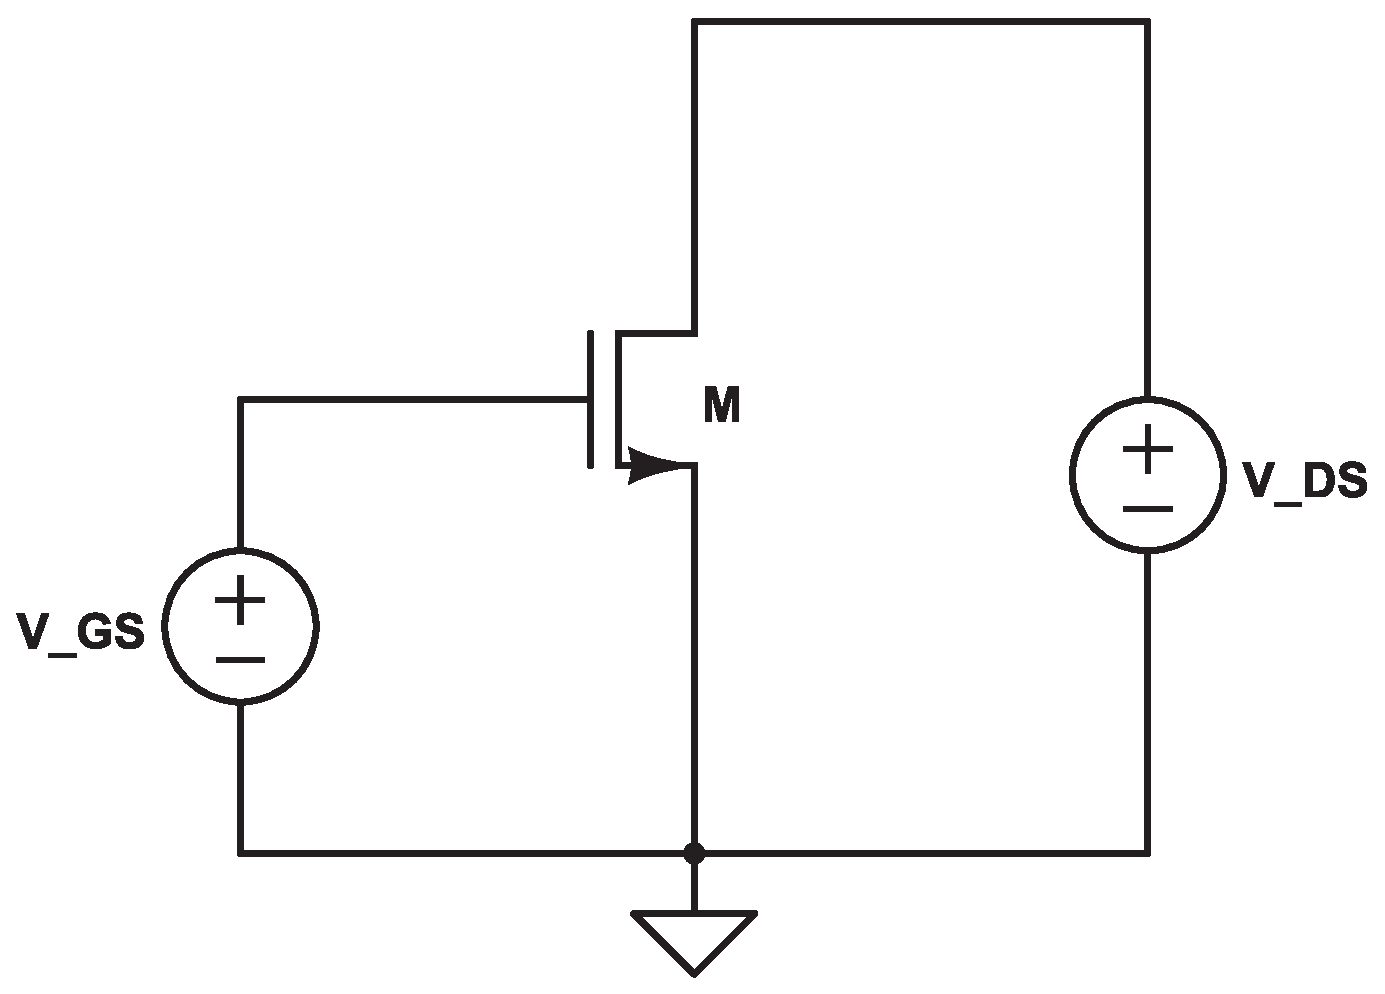
\includegraphics[width=0.5\textwidth]{resource/sim-circuit}
	\caption{Het circuit zoals gebruikt bij simulatie met SPICE}
	\label{fig:ump-sim-circuit}
\end{figure}

In dit circuit geldt als randvoorwaarde dat $V_{SB} = 0$, waaruit volgt dat $V_{T} = V_{T0}$ (zie sectie~\ref{sec:ump-theorie}).
Aan de hand van dit circuit kan vervolgens gesimuleerd worden met SPICE. Voor relevante simulatieresultaten kan als eerste een DC-sweep voor $I_{D}$ met als sweepvariabele $V_{DS}$ en tweede parameter $V_{GS}$ worden uitgevoerd. In figuur~\ref{fig:ump-sim-fig-vds} is het resultaat hiervan weergegeven.
	
\begin{figure}[H]
	\centering
	\setlength\figureheight{0.4\textwidth} 
	\setlength\figurewidth{0.6\textwidth}
	% This file was created by matlab2tikz v0.4.2.
% Copyright (c) 2008--2013, Nico Schlömer <nico.schloemer@gmail.com>
% All rights reserved.
% 
% The latest updates can be retrieved from
%   http://www.mathworks.com/matlabcentral/fileexchange/22022-matlab2tikz
% where you can also make suggestions and rate matlab2tikz.
% 
% 
% 
%
% defining custom colors
\definecolor{mycolor1}{rgb}{0.8,1,0}%
\definecolor{mycolor2}{rgb}{0,1,0.4}%
\definecolor{mycolor3}{rgb}{0,0.4,1}%
\definecolor{mycolor4}{rgb}{0.800000000000001,0,1}%
\definecolor{mycolor5}{rgb}{0.75,0.75,0}%
%
\begin{tikzpicture}

\begin{axis}[%
width=\figurewidth,
height=\figureheight,
scale only axis,
xmin=0,
xmax=6.99999999999998,
xlabel={$V_{DS}$},
ymin=0,
ymax=0.00657962635159492,
ylabel={$I_{D}$},
axis x line*=bottom,
axis y line*=left,
legend style={draw=black,fill=white,legend cell align=left}
]
\addplot [
color=red,
solid
]
table[row sep=crcr]{
0 0\\
0.05 2.63460588030284e-05\\
0.1 4.82380200992338e-05\\
0.15 6.57152995700017e-05\\
0.2 7.88139586802572e-05\\
0.25 8.75671539688483e-05\\
0.3 9.18564983294345e-05\\
0.35 9.37392032938078e-05\\
0.4 9.52351838350296e-05\\
0.45 9.65605140663683e-05\\
0.5 9.77818344836123e-05\\
0.55 9.89303589449264e-05\\
0.6 0.000100023768027313\\
0.65 0.000101073288533371\\
0.7 0.000102086603874341\\
0.75 0.000103069243778009\\
0.8 0.000104025413747877\\
0.85 0.000104958351585083\\
0.9 0.00010587066935841\\
0.95 0.000106764484371524\\
1 0.000107641564682126\\
1.05 0.000108503387309611\\
1.1 0.000109351232822519\\
1.15 0.000110186192614492\\
1.2 0.000111009227111936\\
1.25 0.000111821180325933\\
1.3 0.000112622787128203\\
1.35 0.000113414724182803\\
1.4 0.000114197580842301\\
1.45 0.000114971902803518\\
1.5 0.000115738177555613\\
1.55 0.000116496841656044\\
1.6 0.000117248309834395\\
1.65 0.000117992953164503\\
1.7 0.000118731113616377\\
1.75 0.000119463111332152\\
1.8 0.000120189237350132\\
1.85 0.000120909768156707\\
1.9 0.000121624958410393\\
1.95 0.000122335040941834\\
2 0.000123040226753801\\
2.05 0.000123740755952895\\
2.1 0.000124436788610183\\
2.15 0.000125128528452478\\
2.2 0.000125816150102764\\
2.25 0.000126499799080193\\
2.3 0.000127179650007747\\
2.35 0.000127855833852664\\
2.4 0.00012852851068601\\
2.45 0.000129197767819278\\
2.5 0.00012986377987545\\
2.55 0.000130526634166017\\
2.6 0.000131186461658217\\
2.65 0.000131843349663541\\
2.7 0.00013249741459731\\
2.75 0.000133148758322932\\
2.8 0.000133797468151897\\
2.85 0.000134443631395698\\
2.9 0.000135087335365824\\
2.95 0.000135728667373769\\
3 0.000136367700179107\\
3.05 0.000137004521093331\\
3.1 0.000137639188324101\\
3.15 0.000138271774630994\\
3.2 0.0001389023673255\\
3.25 0.000139531010063365\\
3.3 0.000140157761052251\\
3.35 0.000140782693051733\\
3.4 0.000141405878821388\\
3.45 0.000142027347465046\\
3.5 0.000142647157190368\\
3.55 0.000143265366205014\\
3.6 0.000143882032716647\\
3.65 0.000144497200381011\\
3.69999999999999 0.000145110912853852\\
3.74999999999999 0.000145723228342831\\
3.79999999999999 0.000146334161399864\\
3.84999999999999 0.000146943799336441\\
3.89999999999999 0.000147552142152563\\
3.94999999999999 0.000148159262607805\\
3.99999999999999 0.000148765175254084\\
4.04999999999999 0.000149369923747145\\
4.09999999999999 0.000149973566294648\\
4.14999999999999 0.000150576117448509\\
4.19999999999999 0.000151177620864473\\
4.24999999999999 0.000151778105646372\\
4.29999999999999 0.00015237761544995\\
4.34999999999999 0.000152976164827123\\
4.39999999999999 0.000153573797433637\\
4.44999999999999 0.000154170542373322\\
4.49999999999999 0.000154766443301924\\
4.54999999999999 0.000155361500219442\\
4.59999999999999 0.000155955756781623\\
4.64999999999999 0.000156549242092296\\
4.69999999999999 0.000157141985255294\\
4.74999999999999 0.000157734015374444\\
4.79999999999999 0.000158325347001664\\
4.84999999999999 0.000158916009240784\\
4.89999999999999 0.000159506031195633\\
4.94999999999999 0.000160095441970043\\
4.99999999999999 0.000160684241564013\\
5.04999999999999 0.000161272473633289\\
5.09999999999999 0.000161860167281702\\
5.14999999999999 0.000162447322509252\\
5.19999999999999 0.000163033968419768\\
5.24999999999999 0.000163620134117082\\
5.29999999999999 0.000164205834153108\\
5.34999999999999 0.000164791097631678\\
5.39999999999999 0.000165375939104706\\
5.44999999999999 0.000165960358572192\\
5.49999999999999 0.000166544399689883\\
5.54999999999999 0.000167128077009693\\
5.59999999999999 0.000167711405083537\\
5.64999999999999 0.000168294413015246\\
5.69999999999999 0.000168877086252905\\
5.74999999999999 0.000169459483004175\\
5.79999999999999 0.00017004158871714\\
5.84999999999999 0.000170623432495631\\
5.89999999999999 0.000171205043443479\\
5.94999999999999 0.000171786407008767\\
5.99999999999999 0.000172367581399158\\
6.04999999999999 0.00017294853751082\\
6.09999999999999 0.000173529318999499\\
6.14999999999999 0.000174109925865196\\
6.19999999999999 0.00017469038721174\\
6.24999999999999 0.000175270703039132\\
6.29999999999999 0.000175850902451202\\
6.34999999999999 0.000176430999999866\\
6.39999999999999 0.000177010995685123\\
6.44999999999999 0.000177590904058889\\
6.49999999999998 0.000178170739673078\\
6.54999999999998 0.000178750531631522\\
6.59999999999998 0.000179330265382305\\
6.64999999999998 0.000179909984581172\\
6.69999999999998 0.000180489689228125\\
6.74999999999998 0.000181069379323162\\
6.79999999999998 0.000181649083970115\\
6.84999999999998 0.000182228803168982\\
6.89999999999998 0.000182808566023596\\
6.94999999999998 0.000183388357982039\\
6.99999999999998 0.000183968208148144\\
};
\addlegendentry{$V_{GS}: 1 V$};

\addplot [
color=mycolor1,
solid
]
table[row sep=crcr]{
0 0\\
0.05 7.49292084947228e-05\\
0.1 0.000146480320836417\\
0.15 0.000214678308111615\\
0.2 0.000279545987723395\\
0.25 0.000341104430845007\\
0.3 0.000399373035179451\\
0.35 0.000454369815997779\\
0.4 0.000506111595313996\\
0.45 0.000554614001885057\\
0.5 0.000599891762249172\\
0.55 0.000641958671621978\\
0.6 0.00068082771031186\\
0.65 0.000716511101927608\\
0.7 0.000749020429793745\\
0.75 0.000778366753365844\\
0.8 0.000802196154836565\\
0.85 0.000814971455838531\\
0.9 0.000824656221084297\\
0.95 0.000832951162010431\\
1 0.000840405293274671\\
1.05 0.000847279618028551\\
1.1 0.000853722391184419\\
1.15 0.00085982761811465\\
1.2 0.000865659210830927\\
1.25 0.00087126309517771\\
1.3 0.000876673555467278\\
1.35 0.000881917017977685\\
1.4 0.000887014379259199\\
1.45 0.000891982461325824\\
1.5 0.000896835117600858\\
1.55 0.000901583873201162\\
1.6 0.000906238507013768\\
1.65 0.000910807284526527\\
1.7 0.000915297481697053\\
1.75 0.000919715210329741\\
1.8 0.000924066000152379\\
1.85 0.000928354682400823\\
1.9 0.000932585564441979\\
1.95 0.000936762487981468\\
2 0.000940888829063624\\
2.05 0.000944967789109796\\
2.1 0.000949002045672387\\
2.15 0.000952994276303798\\
2.2 0.000956946809310466\\
2.25 0.000960861740168184\\
2.3 0.000964741047937423\\
2.35 0.000968586537055671\\
2.4 0.000972399895545095\\
2.45 0.00097618269501254\\
2.5 0.000979936448857188\\
2.55 0.000983662321232259\\
2.6 0.000987361650913954\\
2.65 0.000991035718470812\\
2.7 0.000994685455225408\\
2.75 0.000998312025330961\\
2.8 0.00100191636011004\\
2.85 0.00100549927446991\\
2.9 0.00100906181614846\\
2.95 0.00101260468363762\\
3 0.00101612857542932\\
3.05 0.00101963430643082\\
3.1 0.00102312269154936\\
3.15 0.00102659419644624\\
3.2 0.00103004940319806\\
3.25 0.00103348912671208\\
3.3 0.00103691383264959\\
3.35 0.00104032398667187\\
3.4 0.00104372017085552\\
3.45 0.00104710285086185\\
3.5 0.00105047249235213\\
3.55 0.00105382956098765\\
3.6 0.0010571745224297\\
3.65 0.00106050784233958\\
3.69999999999999 0.00106382975354791\\
3.74999999999999 0.00106714060530066\\
3.79999999999999 0.00107044097967446\\
3.84999999999999 0.00107373122591525\\
3.89999999999999 0.00107701146043837\\
3.94999999999999 0.0010802821489051\\
3.99999999999999 0.00108354352414608\\
4.04999999999999 0.0010867960518226\\
4.09999999999999 0.00109003984834999\\
4.14999999999999 0.0010932752629742\\
4.19999999999999 0.00109650264494121\\
4.24999999999999 0.00109972211066633\\
4.29999999999999 0.00110293400939554\\
4.34999999999999 0.00110613857395947\\
4.39999999999999 0.00110933603718877\\
4.44999999999999 0.00111252663191408\\
4.49999999999999 0.00111571059096605\\
4.54999999999999 0.00111888803075999\\
4.59999999999999 0.00112205930054188\\
4.64999999999999 0.00112522463314235\\
4.69999999999999 0.00112838402856141\\
4.74999999999999 0.00113153783604503\\
4.79999999999999 0.00113468628842384\\
4.84999999999999 0.00113782938569784\\
4.89999999999999 0.00114096736069769\\
4.94999999999999 0.00114410056266934\\
4.99999999999999 0.00114722887519747\\
5.04999999999999 0.00115035276394337\\
5.09999999999999 0.00115347211249173\\
5.14999999999999 0.00115658715367317\\
5.19999999999999 0.00115969812031835\\
5.24999999999999 0.00116280512884259\\
5.29999999999999 0.00116590841207653\\
5.34999999999999 0.00116900785360485\\
5.39999999999999 0.00117210380267352\\
5.44999999999999 0.00117519625928253\\
5.49999999999999 0.00117828557267785\\
5.54999999999999 0.00118137162644416\\
5.59999999999999 0.0011844546534121\\
5.64999999999999 0.001187534769997\\
5.69999999999999 0.00119061197619885\\
5.74999999999999 0.00119368662126362\\
5.79999999999999 0.00119675870519131\\
5.84999999999999 0.00119982822798193\\
5.89999999999999 0.00120289553888142\\
5.94999999999999 0.00120596052147448\\
5.99999999999999 0.00120902329217643\\
6.04999999999999 0.00121208420023322\\
6.09999999999999 0.00121514301281422\\
6.14999999999999 0.0012182000791654\\
6.19999999999999 0.00122125528287143\\
6.24999999999999 0.00122430897317827\\
6.29999999999999 0.0012273610336706\\
6.34999999999999 0.00123041158076376\\
6.39999999999999 0.00123346084728837\\
6.44999999999999 0.00123650871682912\\
6.49999999999998 0.00123955542221665\\
6.54999999999998 0.00124260107986629\\
6.59999999999998 0.00124564557336271\\
6.64999999999998 0.00124868925195187\\
6.69999999999998 0.00125173188280314\\
6.74999999999998 0.00125477381516248\\
6.79999999999998 0.00125781504902989\\
6.84999999999998 0.00126085558440536\\
6.89999999999998 0.00126389553770423\\
6.94999999999998 0.00126693502534181\\
6.99999999999998 0.00126997416373342\\
};
\addlegendentry{$V_{GS}: 2 V$};

\addplot [
color=mycolor2,
solid
]
table[row sep=crcr]{
0 0\\
0.05 0.000115335518785287\\
0.1 0.000227671131142415\\
0.15 0.000337028264766559\\
0.2 0.000443426542915404\\
0.25 0.000546884024515748\\
0.3 0.000647417444270104\\
0.35 0.000745042169000953\\
0.4 0.000839772750623524\\
0.45 0.000931622460484505\\
0.5 0.00102060404606164\\
0.55 0.00110672926530242\\
0.6 0.00119000929407775\\
0.65 0.0012704546097666\\
0.7 0.00134807522408664\\
0.75 0.00142288045026362\\
0.8 0.00149487913586199\\
0.85 0.0015640800120309\\
0.9 0.00163049099501222\\
0.95 0.00169411988463253\\
1 0.00175497401505709\\
1.05 0.00181306048762053\\
1.1 0.00186838593799621\\
1.15 0.00190638634376228\\
1.2 0.00193048210348934\\
1.25 0.00195011962205172\\
1.3 0.00196732394397259\\
1.35 0.00198293710127473\\
1.4 0.00199740473181009\\
1.45 0.00201099738478661\\
1.5 0.00202389364130795\\
1.55 0.00203621829859912\\
1.6 0.00204806355759501\\
1.65 0.00205949880182743\\
1.7 0.00207057851366699\\
1.75 0.00208134623244405\\
1.8 0.00209183688275516\\
1.85 0.00210208026692271\\
1.9 0.002112100366503\\
1.95 0.00212191813625395\\
2 0.00213155150413513\\
2.05 0.00214101560413837\\
2.1 0.00215032417327166\\
2.15 0.00215948885306716\\
2.2 0.00216851988807321\\
2.25 0.00217742659151554\\
2.3 0.00218621757812798\\
2.35 0.00219490006566048\\
2.4 0.0022034808062017\\
2.45 0.00221196585334837\\
2.5 0.00222036056220531\\
2.55 0.00222867052070796\\
2.6 0.00223689991980791\\
2.65 0.00224505318328738\\
2.7 0.00225313426926732\\
2.75 0.00226114667020738\\
2.8 0.00226909387856722\\
2.85 0.00227697915397584\\
2.9 0.00228480505757034\\
2.95 0.00229257461614907\\
3 0.00230029015801847\\
3.05 0.00230795424431562\\
3.1 0.00231556897051632\\
3.15 0.00232313643209636\\
3.2 0.00233065849170089\\
3.25 0.00233813747763634\\
3.3 0.00234557455405593\\
3.35 0.00235297158360481\\
3.4 0.00236033019609749\\
3.45 0.00236765202134848\\
3.5 0.00237493822351098\\
3.55 0.00238219019956887\\
3.6 0.002389409346506\\
3.65 0.00239659659564495\\
3.69999999999999 0.00240375334396958\\
3.74999999999999 0.00241088075563312\\
3.79999999999999 0.00241797952912748\\
3.84999999999999 0.00242505106143653\\
3.89999999999999 0.00243209628388286\\
3.94999999999999 0.00243911589495838\\
3.99999999999999 0.00244611082598567\\
4.04999999999999 0.00245308177545667\\
4.09999999999999 0.00246003014035523\\
4.14999999999999 0.00246695592068136\\
4.19999999999999 0.00247386051341891\\
4.24999999999999 0.00248074438422918\\
4.29999999999999 0.0024876082316041\\
4.34999999999999 0.00249445252120495\\
4.39999999999999 0.00250127818435431\\
4.44999999999999 0.0025080859195441\\
4.49999999999999 0.00251487595960498\\
4.54999999999999 0.00252164923585951\\
4.59999999999999 0.00252840598113835\\
4.64999999999999 0.00253514689393342\\
4.69999999999999 0.00254187267273664\\
4.74999999999999 0.00254858355037868\\
4.79999999999999 0.00255528022535145\\
4.84999999999999 0.00256196293048561\\
4.89999999999999 0.00256863236427307\\
4.94999999999999 0.00257528899237514\\
4.99999999999999 0.0025819328147918\\
5.04999999999999 0.00258856476284564\\
5.09999999999999 0.00259518506936729\\
5.14999999999999 0.0026017939671874\\
5.19999999999999 0.00260839215479791\\
5.24999999999999 0.00261497963219881\\
5.29999999999999 0.00262155709788203\\
5.34999999999999 0.00262812478467822\\
5.39999999999999 0.00263468292541802\\
5.44999999999999 0.00264123198576272\\
5.49999999999999 0.00264777219854295\\
5.54999999999999 0.00265430402942002\\
5.59999999999999 0.00266082747839391\\
5.64999999999999 0.00266734324395657\\
5.69999999999999 0.00267385132610798\\
5.74999999999999 0.00268035219050944\\
5.79999999999999 0.00268684606999159\\
5.84999999999999 0.00269333319738507\\
5.89999999999999 0.00269981380552053\\
5.94999999999999 0.00270628836005926\\
5.99999999999999 0.00271275686100125\\
6.04999999999999 0.00271921954117715\\
6.09999999999999 0.00272567686624825\\
6.14999999999999 0.00273212883621454\\
6.19999999999999 0.00273857591673732\\
6.24999999999999 0.00274501834064722\\
6.29999999999999 0.00275145610794425\\
6.34999999999999 0.00275788945145905\\
6.39999999999999 0.00276431883685291\\
6.44999999999999 0.00277074426412582\\
6.49999999999998 0.00277716619893909\\
6.54999999999998 0.00278358440846205\\
6.59999999999998 0.002789999358356\\
6.64999999999998 0.00279641128145158\\
6.69999999999998 0.0028028201777488\\
6.74999999999998 0.00280922651290894\\
6.79999999999998 0.00281563028693199\\
6.84999999999998 0.00282203149981797\\
6.89999999999998 0.00282843085005879\\
6.94999999999998 0.00283482787199318\\
6.99999999999998 0.00284122326411307\\
};
\addlegendentry{$V_{GS}: 3 V$};

\addplot [
color=mycolor3,
solid
]
table[row sep=crcr]{
0 0\\
0.05 0.000152013642946258\\
0.1 0.000301248859614134\\
0.15 0.000447725178673863\\
0.2 0.000591460557188839\\
0.25 0.000732471467927098\\
0.3 0.000870773161295801\\
0.35 0.00100637972354889\\
0.4 0.00113930436782539\\
0.45 0.00126955937594175\\
0.5 0.00139715615659952\\
0.55 0.00152210565283895\\
0.6 0.0016444178763777\\
0.65 0.0017641024896875\\
0.7 0.00188116845674813\\
0.75 0.00199562450870872\\
0.8 0.00210747867822647\\
0.85 0.00221673888154328\\
0.9 0.00232341233640909\\
0.95 0.00242750602774322\\
1 0.00252902670763433\\
1.05 0.00262798089534044\\
1.1 0.00272437487728894\\
1.15 0.00281821400858462\\
1.2 0.00290950457565486\\
1.25 0.00299825146794319\\
1.3 0.00308446027338505\\
1.35 0.00316523713991046\\
1.4 0.00321417511440814\\
1.45 0.00325011112727225\\
1.5 0.00328038237057626\\
1.55 0.00330727314576507\\
1.6 0.00333185330964625\\
1.65 0.00335472635924816\\
1.7 0.00337627273984253\\
1.75 0.00339674996212125\\
1.8 0.00341634219512343\\
1.85 0.00343518680892885\\
1.9 0.00345338857732713\\
1.95 0.00347103085368872\\
2 0.00348818046040833\\
2.05 0.00350489164702594\\
2.1 0.00352121028117836\\
2.15 0.00353717454709113\\
2.2 0.00355281657539308\\
2.25 0.00356816477142274\\
2.3 0.00358324334956706\\
2.35 0.00359807349741459\\
2.4 0.00361267384141684\\
2.45 0.0036270609125495\\
2.5 0.00364124937914312\\
2.55 0.00365525274537504\\
2.6 0.00366908241994679\\
2.65 0.00368274957872927\\
2.7 0.00369626353494823\\
2.75 0.00370963360182941\\
2.8 0.00372286746278405\\
2.85 0.0037359728012234\\
2.9 0.00374895636923611\\
2.95 0.00376182445324957\\
3 0.00377458287402987\\
3.05 0.00378723698668182\\
3.1 0.00379979168064892\\
3.15 0.00381225207820535\\
3.2 0.00382462213747203\\
3.25 0.00383690581656992\\
3.3 0.00384910730645061\\
3.35 0.00386123009957373\\
3.4 0.00387327745556831\\
3.45 0.00388525240123272\\
3.5 0.00389715796336532\\
3.55 0.00390899740159512\\
3.6 0.00392077257856727\\
3.65 0.00393248675391078\\
3.69999999999999 0.00394414179027081\\
3.74999999999999 0.00395574001595378\\
3.79999999999999 0.00396728422492743\\
3.84999999999999 0.00397877534851432\\
3.89999999999999 0.00399021664634347\\
3.94999999999999 0.00400160858407617\\
3.99999999999999 0.00401295395568013\\
4.04999999999999 0.00402425415813923\\
4.09999999999999 0.00403551058843732\\
4.14999999999999 0.00404672464355826\\
4.19999999999999 0.0040578986518085\\
4.24999999999999 0.00406903307884932\\
4.29999999999999 0.00408012978732586\\
4.34999999999999 0.00409119017422199\\
4.39999999999999 0.00410221517086029\\
4.44999999999999 0.00411320570856333\\
4.49999999999999 0.00412416364997625\\
4.54999999999999 0.00413508992642164\\
4.59999999999999 0.00414598546922207\\
4.64999999999999 0.00415685074403882\\
4.69999999999999 0.00416768807917833\\
4.74999999999999 0.00417849700897932\\
4.79999999999999 0.00418927939608693\\
4.84999999999999 0.00420003570616245\\
4.89999999999999 0.00421076687052846\\
4.94999999999999 0.00422147428616881\\
4.99999999999999 0.00423215795308352\\
5.04999999999999 0.00424281880259514\\
5.09999999999999 0.00425345776602626\\
5.14999999999999 0.00426407577469945\\
5.19999999999999 0.004274673294276\\
5.24999999999999 0.00428525079041719\\
5.29999999999999 0.00429580919444561\\
5.34999999999999 0.00430634943768382\\
5.39999999999999 0.00431687198579311\\
5.44999999999999 0.00432737683877349\\
5.49999999999999 0.00433786539360881\\
5.54999999999999 0.00434833765029907\\
5.59999999999999 0.00435879500582814\\
5.64999999999999 0.00436923699453473\\
5.69999999999999 0.00437966454774141\\
5.74999999999999 0.00439007859677076\\
5.79999999999999 0.00440047914162278\\
5.84999999999999 0.00441086664795876\\
5.89999999999999 0.00442124158143997\\
5.94999999999999 0.00443160487338901\\
5.99999999999999 0.00444195698946714\\
6.04999999999999 0.0044522974640131\\
6.09999999999999 0.00446262769401073\\
6.14999999999999 0.00447294814512134\\
6.19999999999999 0.00448325835168362\\
6.24999999999999 0.00449355924502015\\
6.29999999999999 0.00450385129079223\\
6.34999999999999 0.00451413495466113\\
6.39999999999999 0.00452441023662686\\
6.44999999999999 0.00453467760235071\\
6.49999999999998 0.00454493798315525\\
6.54999999999998 0.00455519091337919\\
6.59999999999998 0.00456543732434511\\
6.64999999999998 0.00457567721605301\\
6.69999999999998 0.00458591105416417\\
6.74999999999998 0.00459613930433989\\
6.79999999999998 0.00460636196658015\\
6.84999999999998 0.00461657950654626\\
6.89999999999998 0.00462679238989949\\
6.94999999999998 0.00463700061663985\\
6.99999999999998 0.00464720465242863\\
};
\addlegendentry{$V_{GS}: 4 V$};

\addplot [
color=mycolor4,
solid
]
table[row sep=crcr]{
0 0\\
0.05 0.000186325123650022\\
0.1 0.000370025110896677\\
0.15 0.000551118282601237\\
0.2 0.000729621504433453\\
0.25 0.000905550143215805\\
0.3 0.00107891857624054\\
0.35 0.00124974001664668\\
0.4 0.00141802674625069\\
0.45 0.00158379029016942\\
0.5 0.0017470414750278\\
0.55 0.00190779031254351\\
0.6 0.00206604646518826\\
0.65 0.00222181878052652\\
0.7 0.00237511587329209\\
0.75 0.00252594565972686\\
0.8 0.00267431582324207\\
0.85 0.00282023381441832\\
0.9 0.00296370615251362\\
0.95 0.00310473958961666\\
1 0.00324334064498544\\
1.05 0.00337951490655541\\
1.1 0.00351326842792332\\
1.15 0.00364460679702461\\
1.2 0.00377353490330279\\
1.25 0.00390005833469331\\
1.3 0.00402418151497841\\
1.35 0.00414590956643224\\
1.4 0.00426524644717574\\
1.45 0.00438219727948308\\
1.5 0.00449676578864455\\
1.55 0.00458967918530107\\
1.6 0.00464787520468235\\
1.65 0.00469437940046191\\
1.7 0.00473469868302345\\
1.75 0.00477103190496564\\
1.8 0.00480452459305525\\
1.85 0.00483586173504591\\
1.9 0.0048654917627573\\
1.95 0.00489372760057449\\
2 0.00492079742252827\\
2.05 0.0049468744546175\\
2.1 0.00497209234163165\\
2.15 0.00499655865132809\\
2.2 0.00502035999670625\\
2.25 0.00504356762394309\\
2.3 0.00506624253466725\\
2.35 0.00508843408897519\\
2.4 0.0051101865246892\\
2.45 0.00513153662905097\\
2.5 0.00515251746401191\\
2.55 0.00517315790057182\\
2.6 0.00519348215311766\\
2.65 0.00521351350471377\\
2.7 0.00523327151313424\\
2.75 0.00525277433916926\\
2.8 0.00527203781530261\\
2.85 0.00529107730835676\\
2.9 0.00530990492552519\\
2.95 0.00532853370532393\\
3 0.0053469748236239\\
3.05 0.00536523805931211\\
3.1 0.00538333272561431\\
3.15 0.00540126767009497\\
3.2 0.00541905080899596\\
3.25 0.00543668959289789\\
3.3 0.00545419100672007\\
3.35 0.00547156156972051\\
3.4 0.00548880686983466\\
3.45 0.00550593296065927\\
3.5 0.00552294496446848\\
3.55 0.00553984753787518\\
3.6 0.00555664580315351\\
3.65 0.00557334395125508\\
3.69999999999999 0.00558994570747018\\
3.74999999999999 0.00560645572841167\\
3.79999999999999 0.00562287727370858\\
3.84999999999999 0.00563921360298991\\
3.89999999999999 0.00565546797588468\\
3.94999999999999 0.00567164411768317\\
3.99999999999999 0.00568774482235312\\
4.04999999999999 0.00570377241820097\\
4.09999999999999 0.00571973016485572\\
4.14999999999999 0.00573562039062381\\
4.19999999999999 0.00575144542381167\\
4.24999999999999 0.00576720805838704\\
4.29999999999999 0.00578291015699506\\
4.34999999999999 0.00579855358228087\\
4.39999999999999 0.00581414112821221\\
4.44999999999999 0.00582967419177294\\
4.49999999999999 0.00584515510126948\\
4.54999999999999 0.00586058478802443\\
4.59999999999999 0.00587596604600549\\
4.64999999999999 0.00589130027219653\\
4.69999999999999 0.00590658839792013\\
4.74999999999999 0.00592183275148273\\
4.79999999999999 0.00593703472986817\\
4.84999999999999 0.00595219526439905\\
4.89999999999999 0.00596731575205922\\
4.94999999999999 0.00598239805549383\\
4.99999999999999 0.00599744357168674\\
5.04999999999999 0.00601245276629925\\
5.09999999999999 0.00602742750197649\\
5.14999999999999 0.00604236824437976\\
5.19999999999999 0.0060572768561542\\
5.24999999999999 0.0060721542686224\\
5.29999999999999 0.00608700141310692\\
5.34999999999999 0.00610181922093034\\
5.39999999999999 0.00611660862341523\\
5.44999999999999 0.00613137055188417\\
5.49999999999999 0.00614610640332103\\
5.54999999999999 0.00616081664338708\\
5.59999999999999 0.0061755022034049\\
5.64999999999999 0.00619016401469707\\
5.69999999999999 0.00620480300858617\\
5.74999999999999 0.00621941965073347\\
5.79999999999999 0.00623401533812284\\
5.84999999999999 0.00624859007075429\\
5.89999999999999 0.00626314524561167\\
5.94999999999999 0.00627768132835627\\
5.99999999999999 0.00629219878464937\\
6.04999999999999 0.00630669854581356\\
6.09999999999999 0.00632118107751012\\
6.14999999999999 0.00633564731106162\\
6.19999999999999 0.00635009817779064\\
6.24999999999999 0.00636453321203589\\
6.29999999999999 0.00637895427644253\\
6.34999999999999 0.00639336090534925\\
6.39999999999999 0.00640775449573994\\
6.44999999999999 0.00642213504761457\\
6.49999999999998 0.00643650349229574\\
6.54999999999998 0.00645086029544473\\
6.59999999999998 0.00646520592272282\\
6.64999999999998 0.00647954037413001\\
6.69999999999998 0.00649386504665017\\
6.74999999999998 0.0065081799402833\\
6.79999999999998 0.00652248598635197\\
6.84999999999998 0.00653678271919489\\
6.89999999999998 0.00655107153579593\\
6.94999999999998 0.00656535243615508\\
6.99999999999998 0.00657962635159492\\
};
\addlegendentry{$V_{GS}: 5 V$};

\addplot [
color=mycolor5,
solid
]
table[row sep=crcr]{
0 0\\
0.05 5.12573363084812e-06\\
0.1 2.05029345233925e-05\\
0.15 4.6131602677633e-05\\
0.2 8.20117380935699e-05\\
0.25 0.000128143340771203\\
0.3 0.000184526410710532\\
0.35 0.000251160947911558\\
0.4 0.000328046952374279\\
0.45 0.000415184424098697\\
0.5 0.000512573363084812\\
0.55 0.000620213769332622\\
0.6 0.000738105642842129\\
0.65 0.000866248983613332\\
0.7 0.00100464379164623\\
0.75 0.00115329006694083\\
0.8 0.00131218780949712\\
0.85 0.00148133701931511\\
0.9 0.00166073769639479\\
0.95 0.00185038984073617\\
1 0.00205029345233925\\
1.05 0.00226044853120402\\
1.1 0.00248085507733049\\
1.15 0.00271151309071865\\
1.2 0.00295242257136851\\
1.25 0.00320358351928007\\
1.3 0.00346499593445333\\
1.35 0.00373665981688828\\
1.4 0.00401857516658492\\
1.45 0.00431074198354326\\
1.5 0.0046131602677633\\
1.55 0.00492583001924504\\
1.6 0.00524875123798847\\
1.65 0.0055819239239936\\
1.7 0.00592534807726042\\
1.75 0.00627902369778894\\
1.8 0.00664295078557916\\
1.85 0.00701712934063107\\
1.9 0.00740155936294468\\
1.95 0.00779624085251998\\
2 0.00820117380935699\\
2.05 0.00861635823345568\\
2.1 0.00904179412481608\\
2.15 0.00947748148343817\\
2.2 0.00992342030932195\\
2.25 0.0103796106024674\\
2.3 0.0108460523628746\\
2.35 0.0113227455905435\\
2.4 0.0118096902854741\\
2.45 0.0123068864476663\\
2.5 0.0128143340771203\\
2.55 0.0133320331738359\\
2.6 0.0138599837378133\\
2.65 0.0143981857690524\\
2.7 0.0149466392675531\\
2.75 0.0155053442333156\\
2.8 0.0160743006663397\\
2.85 0.0166535085666255\\
2.9 0.0172429679341731\\
2.95 0.0178426787689823\\
3 0.0184526410710532\\
3.05 0.0190728548403858\\
3.1 0.0197033200769802\\
3.15 0.0203440367808362\\
3.2 0.0209950049519539\\
3.25 0.0216562245903333\\
3.3 0.0223276956959744\\
3.35 0.0230094182688772\\
3.4 0.0237013923090417\\
3.45 0.0244036178164679\\
3.5 0.0251160947911558\\
3.55 0.0258388232331053\\
3.6 0.0265718031423166\\
3.65 0.0273150345187896\\
3.69999999999999 0.0280685173625241\\
3.74999999999999 0.0288322516735205\\
3.79999999999999 0.0296062374517786\\
3.84999999999999 0.0303904746972983\\
3.89999999999999 0.0311849634100798\\
3.94999999999999 0.0319897035901229\\
3.99999999999999 0.0328046952374278\\
4.04999999999999 0.0336299383519943\\
4.09999999999999 0.0344654329338226\\
4.14999999999999 0.0353111789829125\\
4.19999999999999 0.0361671764992641\\
4.24999999999999 0.0370334254828775\\
4.29999999999999 0.0379099259337525\\
4.34999999999999 0.0387966778518892\\
4.39999999999999 0.0396936812372876\\
4.44999999999999 0.0406009360899477\\
4.49999999999999 0.0415184424098696\\
4.54999999999999 0.0424462001970531\\
4.59999999999999 0.0433842094514983\\
4.64999999999999 0.0443324701732052\\
4.69999999999999 0.0452909823621738\\
4.74999999999999 0.0462597460184041\\
4.79999999999999 0.047238761141896\\
4.84999999999999 0.0482280277326497\\
4.89999999999999 0.0492275457906651\\
4.94999999999999 0.0502373153159422\\
4.99999999999999 0.051257336308481\\
5.04999999999999 0.0522876087682814\\
5.09999999999999 0.0533281326953436\\
5.14999999999999 0.0543789080896674\\
5.19999999999999 0.055439934951253\\
5.24999999999999 0.0565112132801003\\
5.29999999999999 0.0575927430762092\\
5.34999999999999 0.0586845243395799\\
5.39999999999999 0.0597865570702122\\
5.44999999999999 0.0608988412681062\\
5.49999999999999 0.062021376933262\\
5.54999999999999 0.0631541640656794\\
5.59999999999999 0.0642972026653585\\
5.64999999999999 0.0654504927322993\\
5.69999999999999 0.0666140342665019\\
5.74999999999999 0.0677878272679661\\
5.79999999999999 0.068971871736692\\
5.84999999999999 0.0701661676726796\\
5.89999999999999 0.0713707150759289\\
5.94999999999999 0.0725855139464399\\
5.99999999999999 0.0738105642842126\\
6.04999999999999 0.075045866089247\\
6.09999999999999 0.0762914193615431\\
6.14999999999999 0.0775472241011009\\
6.19999999999999 0.0788132803079204\\
6.24999999999999 0.0800895879820016\\
6.29999999999999 0.0813761471233444\\
6.34999999999999 0.082672957731949\\
6.39999999999999 0.0839800198078152\\
6.44999999999999 0.0852973333509433\\
6.49999999999998 0.0866248983613326\\
6.54999999999998 0.087962714838984\\
6.59999999999998 0.089310782783897\\
6.64999999999998 0.0906691021960718\\
6.69999999999998 0.0920376730755082\\
6.74999999999998 0.0934164954222063\\
6.79999999999998 0.0948055692361662\\
6.84999999999998 0.0962048945173877\\
6.89999999999998 0.0976144712658709\\
6.94999999999998 0.0990342994816159\\
6.99999999999998 0.100464379164622\\
};
\addlegendentry{$V_{DS} \approx V_{GS} - V_{T}$};

\end{axis}
\end{tikzpicture}%
	\caption{SPICE-simulatie: $I_{D}$ uitgezet tegen $V_{DS}$ met vijf verschillende waarden voor $V_{GS}$. De lijn $V_{DS} \approx V_{GS} - V_{T}$ is een gefitte parabool en dient dus slechts als indicatie.}
	\label{fig:ump-sim-fig-vds}
\end{figure}

Uit deze simulatie kan de belangrijkste informatie worden gehaald om de vereiste parameters te bepalen, aan de hand van vergelijking~\ref{eq:ump-cmos-model-rab}. Vervolgens kan een aantal relevante datapunten in een tabel gezet worden, voor gebruik in vergelijking vergelijking~\ref{eq:ump-cmos-model-rab}, zie hiervoor tabel~\ref{tab:ump-sim-tab-vds}. De werkgebieden per datapunten zijn aannames, gemaakt aan de hand van figuur~\ref{fig:ump-sim-fig-vds}. Een daadwerkelijke waarde voor bijvoorbeeld $V_{DSAT}$ moet immers nog bepaald worden. Er is bewust gekozen voor waarden van $V_{GS}$ rond de 5 V, aangezien dit de voedingsspanning ($V_{DD}$) van de uiteindelijk te gebruiken Sea-of-Gates chip is.

\begin{table}[h]
	\centering
	\caption{Enige relevante waarden uit de simulatie van figuur \ref{fig:ump-sim-fig-vds}}
	\label{tab:ump-sim-tab-vds}
	\begin{tabular}{|c|c|c|c|c|} 	
		\hline
		Datapunt & $V_{GS}$ & $V_{DS}$ & $I_{D}$ & Werkgebied \\
		\hline
		1 & 4 V & 2.4 V & 3.775 mA & Verzadiging \\
		\hline
		2 & 4 V & 1.8 V & 3.416 mA & Verzadiging \\
		\hline
		3 & 5 V & 1.8 V & 4.805 mA & Verzadiging \\
		\hline
		4 & 5 V & 5 V & 5.997 mA & Snelheidsverzadiging \\
		\hline	
	\end{tabular}
\end{table}

Daarnaast kan ook een DC-sweep voor $I_{D}$ met als sweepvariabele $V_{GS}$ en als tweede parameter $V_{DS}$ worden uitgevoerd. De resultaten van deze simulatie is te vinden in figuur~\ref{fig:ump-sim-fig-vgs}.

\begin{figure}[H]
	\centering
	\setlength\figureheight{0.4\textwidth} 
	\setlength\figurewidth{0.6\textwidth}
	% This file was created by matlab2tikz v0.4.2.
% Copyright (c) 2008--2013, Nico Schlömer <nico.schloemer@gmail.com>
% All rights reserved.
% 
% The latest updates can be retrieved from
%   http://www.mathworks.com/matlabcentral/fileexchange/22022-matlab2tikz
% where you can also make suggestions and rate matlab2tikz.
% 
% 
% 
%
% defining custom colors
\definecolor{mycolor1}{rgb}{0.8,1,0}%
\definecolor{mycolor2}{rgb}{0,1,0.4}%
\definecolor{mycolor3}{rgb}{0,0.4,1}%
\definecolor{mycolor4}{rgb}{0.800000000000001,0,1}%
%
\begin{tikzpicture}

\begin{axis}[%
width=\figurewidth,
height=\figureheight,
scale only axis,
xmin=0,
xmax=5,
xlabel={$\text{V}_{\text{DS}}$},
ymin=0,
ymax=0.006,
ylabel={$\text{I}_{\text{D}}$},
axis x line*=bottom,
axis y line*=left,
legend style={draw=black,fill=white,legend cell align=left}
]
\addplot [
color=red,
solid
]
table[row sep=crcr]{
0 1.0100000263219e-12\\
0.05 1.0100000263219e-12\\
0.1 1.0100000263219e-12\\
0.15 1.0100000263219e-12\\
0.2 1.0100000263219e-12\\
0.25 1.0100000263219e-12\\
0.3 1.0100000263219e-12\\
0.35 1.0100000263219e-12\\
0.4 1.0100000263219e-12\\
0.45 1.0100000263219e-12\\
0.5 1.0100000263219e-12\\
0.55 1.0100000263219e-12\\
0.6 1.5014289544979e-07\\
0.65 3.16215050588653e-06\\
0.7 1.00194811238907e-05\\
0.75 2.06770528166089e-05\\
0.8 3.38614954671357e-05\\
0.85 4.90048551000655e-05\\
0.9 6.64367325953208e-05\\
0.95 8.6021980678197e-05\\
1 0.000107641564682126\\
1.05 0.000131187989609316\\
1.1 0.000156562600750476\\
1.15 0.000183673648280092\\
1.2 0.000212435144931078\\
1.25 0.000242765905568376\\
1.3 0.000274588936008513\\
1.35 0.000307830836391076\\
1.4 0.000342421553796157\\
1.45 0.000378293887479231\\
1.5 0.000415383226936683\\
1.55 0.000453627435490489\\
1.6 0.000492966442834586\\
1.65 0.000533342128619552\\
1.7 0.0005746980314143\\
1.75 0.000616979144979268\\
1.8 0.000660131685435772\\
1.85 0.000704102742020041\\
1.9 0.000748840102460235\\
1.95 0.000794291670899838\\
2 0.000840405293274671\\
2.05 0.000887127942405641\\
2.1 0.000934405135922134\\
2.15 0.000982180004939437\\
2.2 0.00103039166424423\\
2.25 0.00107897387351841\\
2.3 0.00112785154487938\\
2.35 0.00117693655192852\\
2.4 0.00122611946426332\\
2.45 0.001275256392546\\
2.5 0.00132413930259645\\
2.55 0.00137242884375155\\
2.6 0.00141944875940681\\
2.65 0.00146349414717406\\
2.7 0.00150597305037081\\
2.75 0.00154815602581948\\
2.8 0.00159005343448371\\
2.85 0.0016316749388352\\
2.9 0.00167302985209972\\
2.95 0.00171412678901106\\
3 0.00175497401505709\\
3.05 0.00179557933006436\\
3.1 0.0018359498353675\\
3.15 0.00187609274871647\\
3.2 0.0019160145893693\\
3.25 0.00195572152733803\\
3.3 0.00199521984905005\\
3.35 0.00203451467677951\\
3.4 0.00207361206412315\\
3.45 0.00211251666769385\\
3.5 0.00215123360976577\\
3.55 0.00218976777978241\\
3.6 0.00222812336869538\\
3.65 0.00226630480028689\\
3.69999999999999 0.00230431626550853\\
3.74999999999999 0.00234216172248125\\
3.79999999999999 0.00237984512932599\\
3.84999999999999 0.00241736974567175\\
3.89999999999999 0.00245473929680884\\
3.94999999999999 0.00249195727519691\\
3.99999999999999 0.00252902670763433\\
4.04999999999999 0.00256595085375011\\
4.09999999999999 0.00260273274034262\\
4.14999999999999 0.00263937516137958\\
4.19999999999999 0.00267588091082871\\
4.24999999999999 0.00271225278265774\\
4.29999999999999 0.00274849310517311\\
4.34999999999999 0.00278460490517318\\
4.39999999999999 0.00282059004530311\\
4.44999999999999 0.00285645131953061\\
4.49999999999999 0.00289219082333148\\
4.54999999999999 0.00292781088501215\\
4.59999999999999 0.00296331336721778\\
4.64999999999999 0.00299870036542416\\
4.69999999999999 0.00303397420793772\\
4.74999999999999 0.00306913652457297\\
4.79999999999999 0.0031041894108057\\
4.84999999999999 0.00313913426361978\\
4.89999999999999 0.00317397341132164\\
4.94999999999999 0.00320870825089514\\
4.99999999999999 0.00324334064498544\\
};
\addlegendentry{$\text{V}_{\text{DS}}\text{: 1 V}$};

\addplot [
color=mycolor1,
solid
]
table[row sep=crcr]{
0 2.0100000223261e-12\\
0.05 2.0100000223261e-12\\
0.1 2.0100000223261e-12\\
0.15 2.0100000223261e-12\\
0.2 2.0100000223261e-12\\
0.25 2.0100000223261e-12\\
0.3 2.0100000223261e-12\\
0.35 2.0100000223261e-12\\
0.4 2.0100000223261e-12\\
0.45 2.0100000223261e-12\\
0.5 2.0100000223261e-12\\
0.55 2.0100000223261e-12\\
0.6 6.21847959791921e-07\\
0.65 4.97702603752259e-06\\
0.7 1.34689662445453e-05\\
0.75 2.60522465396207e-05\\
0.8 4.06464750994928e-05\\
0.85 5.76944912609179e-05\\
0.9 7.71966952015646e-05\\
0.95 9.90182961686514e-05\\
1 0.000123040226753801\\
1.05 0.000149154991959222\\
1.1 0.000177263966179453\\
1.15 0.000207275690627284\\
1.2 0.000239104687352665\\
1.25 0.000272670586127788\\
1.3 0.000307897542370483\\
1.35 0.000344713684171438\\
1.4 0.000383050821255893\\
1.45 0.000422844052081928\\
1.5 0.000464031647425145\\
1.55 0.00050655473023653\\
1.6 0.000550357217434794\\
1.65 0.000595385557971895\\
1.7 0.00064158852910623\\
1.75 0.000688917411025614\\
1.8 0.000737325521185994\\
1.85 0.000786768330726773\\
1.9 0.000837203289847821\\
1.95 0.000888589769601822\\
2 0.000940888829063624\\
2.05 0.000994063448160887\\
2.1 0.00104807794559747\\
2.15 0.0011028986191377\\
2.2 0.00115849287249148\\
2.25 0.00121482962276787\\
2.3 0.00127187941689044\\
2.35 0.00132961373310536\\
2.4 0.00138800556305796\\
2.45 0.00144702871330082\\
2.5 0.00150665850378573\\
2.55 0.0015668710693717\\
2.6 0.00162764359265566\\
2.65 0.00168895442038774\\
2.7 0.00175078259781003\\
2.75 0.00181310810148716\\
2.8 0.00187591172289103\\
2.85 0.00193917518481612\\
2.9 0.00200288067571819\\
2.95 0.00206701154820621\\
3 0.00213155150413513\\
3.05 0.00219648494385183\\
3.1 0.00226179673336446\\
3.15 0.00232747290283442\\
3.2 0.00239349971525371\\
3.25 0.00245986343361437\\
3.3 0.00252655171789229\\
3.35 0.00259355246089399\\
3.4 0.002660853555426\\
3.45 0.00272844405844808\\
3.5 0.00279631279408932\\
3.55 0.00286444928497076\\
3.6 0.00293284351937473\\
3.65 0.00300148595124483\\
3.69999999999999 0.00307036680169404\\
3.74999999999999 0.00313947745598853\\
3.79999999999999 0.00320880906656384\\
3.84999999999999 0.00327835301868618\\
3.89999999999999 0.00334810162894428\\
3.94999999999999 0.00341804651543498\\
3.99999999999999 0.00348818046040833\\
4.04999999999999 0.00355849601328373\\
4.09999999999999 0.00362898618914187\\
4.14999999999999 0.00369964400306344\\
4.19999999999999 0.00377046316862106\\
4.24999999999999 0.00384143693372607\\
4.29999999999999 0.00391255924478173\\
4.34999999999999 0.00398382358253002\\
4.39999999999999 0.00405522529035807\\
4.44999999999999 0.00412675738334656\\
4.49999999999999 0.00419841520488262\\
4.54999999999999 0.0042701936326921\\
4.59999999999999 0.00434208661317825\\
4.64999999999999 0.0044140899553895\\
4.69999999999999 0.00448619807139039\\
4.74999999999999 0.00455840677022934\\
4.79999999999999 0.00463071092963219\\
4.84999999999999 0.00470310635864735\\
4.89999999999999 0.00477558886632323\\
4.94999999999999 0.00484815379604697\\
4.99999999999999 0.00492079742252827\\
};
\addlegendentry{$\text{V}_{\text{DS}}\text{: 2 V}$};

\addplot [
color=mycolor2,
solid
]
table[row sep=crcr]{
0 3.01000001833029e-12\\
0.05 3.01000001833029e-12\\
0.1 3.01000001833029e-12\\
0.15 3.01000001833029e-12\\
0.2 3.01000001833029e-12\\
0.25 3.01000001833029e-12\\
0.3 3.01000001833029e-12\\
0.35 3.01000001833029e-12\\
0.4 3.01000001833029e-12\\
0.45 3.01000001833029e-12\\
0.5 3.01000001833029e-12\\
0.55 3.01000001833029e-12\\
0.6 1.25803285300208e-06\\
0.65 6.79662207403453e-06\\
0.7 1.6720594430808e-05\\
0.75 3.07796326524112e-05\\
0.8 4.67087447759695e-05\\
0.85 6.53814859106205e-05\\
0.9 8.66380214574747e-05\\
0.95 0.000110340784885921\\
1 0.000136367700179107\\
1.05 0.000164608150953427\\
1.1 0.000194960433873348\\
1.15 0.000227330092457123\\
1.2 0.000261628738371655\\
1.25 0.000297773163765669\\
1.3 0.000335684831952676\\
1.35 0.000375289237126708\\
1.4 0.000416515686083585\\
1.45 0.000459296890767291\\
1.5 0.000503568851854652\\
1.55 0.000549270422197878\\
1.6 0.000596343481447548\\
1.65 0.000644732324872166\\
1.7 0.000694383983500302\\
1.75 0.0007452477584593\\
1.8 0.000797275279182941\\
1.85 0.000850420328788459\\
1.9 0.000904638669453561\\
1.95 0.000959888217039406\\
2 0.00101612857542932\\
2.05 0.00107332121115178\\
2.1 0.00113142933696508\\
2.15 0.00119041767902672\\
2.2 0.00125025259330869\\
2.25 0.00131090194918215\\
2.3 0.00137233489658684\\
2.35 0.00143452209886163\\
2.4 0.00149743538349867\\
2.45 0.00156104774214327\\
2.5 0.00162533356342465\\
2.55 0.00169026805087924\\
2.6 0.00175582768861204\\
2.65 0.00182198989205062\\
2.7 0.00188873300794512\\
2.75 0.00195603631436825\\
2.8 0.00202388013713062\\
2.85 0.00209224526770413\\
2.9 0.00216111354529858\\
2.95 0.00223046727478504\\
3 0.00230029015801847\\
3.05 0.00237056612968445\\
3.1 0.00244127935729921\\
3.15 0.0025124151725322\\
3.2 0.00258395983837545\\
3.25 0.00265589915215969\\
3.3 0.00272822030819952\\
3.35 0.00280091096647084\\
3.4 0.00287395855411887\\
3.45 0.00294735189527273\\
3.5 0.00302107958123088\\
3.55 0.00309513113461435\\
3.6 0.00316949607804418\\
3.65 0.00324416439980268\\
3.69999999999999 0.00331912678666413\\
3.74999999999999 0.0033943741582334\\
3.79999999999999 0.00346989720128477\\
3.84999999999999 0.00354568753391504\\
3.89999999999999 0.00362173723988235\\
3.94999999999999 0.00369803817011416\\
3.99999999999999 0.00377458287402987\\
4.04999999999999 0.00385136366821826\\
4.09999999999999 0.00392837356775999\\
4.14999999999999 0.0040056062862277\\
4.19999999999999 0.00408305460587144\\
4.24999999999999 0.00416071200743318\\
4.29999999999999 0.00423857290297747\\
4.34999999999999 0.00431663123890758\\
4.39999999999999 0.00439488096162677\\
4.44999999999999 0.0044733164831996\\
4.49999999999999 0.00455193314701319\\
4.54999999999999 0.00463072489947081\\
4.59999999999999 0.00470968708395958\\
4.64999999999999 0.00478881550952792\\
4.69999999999999 0.0048681041225791\\
4.74999999999999 0.0049475496634841\\
4.79999999999999 0.00502714747563004\\
4.84999999999999 0.00510689243674278\\
4.89999999999999 0.00518678175285459\\
4.94999999999999 0.00526681030169129\\
4.99999999999999 0.0053469748236239\\
};
\addlegendentry{$\text{V}_{\text{DS}}\text{: 3 V}$};

\addplot [
color=mycolor3,
solid
]
table[row sep=crcr]{
0 4.00999979749406e-12\\
0.05 4.00999979749406e-12\\
0.1 4.00999979749406e-12\\
0.15 4.00999979749406e-12\\
0.2 4.00999979749406e-12\\
0.25 4.00999979749406e-12\\
0.3 4.00999979749406e-12\\
0.35 4.00999979749406e-12\\
0.4 4.00999979749406e-12\\
0.45 4.00999979749406e-12\\
0.5 4.00999979749406e-12\\
0.55 4.00999979749406e-12\\
0.6 2.00291310648026e-06\\
0.65 8.64114190335386e-06\\
0.7 1.98946072487161e-05\\
0.75 3.51273811247665e-05\\
0.8 5.24327842867933e-05\\
0.85 7.26019279682077e-05\\
0.9 9.5471870736219e-05\\
0.95 0.00012090152449673\\
1 0.000148765175254084\\
1.05 0.00017894858319778\\
1.1 0.000211346516152844\\
1.15 0.000245861068833619\\
1.2 0.000282400549622253\\
1.25 0.000320878549246117\\
1.3 0.000361213402356952\\
1.35 0.000403327750973403\\
1.4 0.000447147962404415\\
1.45 0.00049260415835306\\
1.5 0.000539629545528442\\
1.55 0.000588160706683993\\
1.6 0.000638136931229383\\
1.65 0.000689500360749662\\
1.7 0.000742195814382285\\
1.75 0.000796170381363481\\
1.8 0.000851373770274222\\
1.85 0.00090775778517127\\
1.9 0.000965276383794844\\
1.95 0.00102388567756861\\
2 0.00108354352414608\\
2.05 0.00114420987665653\\
2.1 0.00120584631804377\\
2.15 0.00126841606106609\\
2.2 0.00133188418112695\\
2.25 0.00139621691778302\\
2.3 0.0014613822568208\\
2.35 0.00152734958101064\\
2.4 0.00159408955369145\\
2.45 0.00166157400235534\\
2.5 0.00172977591864765\\
2.55 0.00179866992402822\\
2.6 0.00186823098920286\\
2.65 0.0019384358311072\\
2.7 0.00200926186516881\\
2.75 0.00208068732172251\\
2.8 0.00215269136242568\\
2.85 0.00222525442950428\\
2.9 0.0022983574308455\\
2.95 0.00237198197282851\\
3 0.00244611082598567\\
3.05 0.00252072676084936\\
3.1 0.0025958139449358\\
3.15 0.00267135701142251\\
3.2 0.00274734105914831\\
3.25 0.00282375165261328\\
3.3 0.00290057552047074\\
3.35 0.00297779915854335\\
3.4 0.00305540999397635\\
3.45 0.00313339591957629\\
3.5 0.00321174506098032\\
3.55 0.00329044670797884\\
3.6 0.00336948968470097\\
3.65 0.00344886374659836\\
3.69999999999999 0.00352855864912272\\
3.74999999999999 0.00360856484621763\\
3.79999999999999 0.00368887325748801\\
3.84999999999999 0.00376947480253875\\
3.89999999999999 0.00385036109946668\\
3.94999999999999 0.00393152330070734\\
3.99999999999999 0.00401295395568013\\
4.04999999999999 0.00409464491531253\\
4.09999999999999 0.00417658919468522\\
4.14999999999999 0.00425877934321761\\
4.19999999999999 0.00434120837599039\\
4.24999999999999 0.00442386977374554\\
4.29999999999999 0.00450675701722503\\
4.34999999999999 0.00458986358717084\\
4.39999999999999 0.00467318389564753\\
4.44999999999999 0.00475671235471964\\
4.49999999999999 0.00484044244512916\\
4.54999999999999 0.00492436904460192\\
4.59999999999999 0.00500848703086376\\
4.64999999999999 0.00509279174730182\\
4.69999999999999 0.00517727760598063\\
4.74999999999999 0.00526193995028734\\
4.79999999999999 0.00534677458927035\\
4.84999999999999 0.00543177640065551\\
4.89999999999999 0.00551694165915251\\
4.94999999999999 0.00560226570814848\\
4.99999999999999 0.00568774482235312\\
};
\addlegendentry{$\text{V}_{\text{DS}}\text{: 4 V}$};

\addplot [
color=mycolor4,
solid
]
table[row sep=crcr]{
0 5.00999979349825e-12\\
0.05 5.00999979349825e-12\\
0.1 5.00999979349825e-12\\
0.15 5.00999979349825e-12\\
0.2 5.00999979349825e-12\\
0.25 5.00999979349825e-12\\
0.3 5.00999979349825e-12\\
0.35 5.00999979349825e-12\\
0.4 5.00999979349825e-12\\
0.45 5.00999979349825e-12\\
0.5 5.00999979349825e-12\\
0.55 1.44762148934774e-08\\
0.6 2.832834070432e-06\\
0.65 1.05232902569696e-05\\
0.7 2.30493133130949e-05\\
0.75 3.93691916542593e-05\\
0.8 5.79878396820277e-05\\
0.85 7.9585071944166e-05\\
0.9 0.000103994309029076\\
0.95 0.000131070570205338\\
1 0.000160684241564013\\
1.05 0.00019271727069281\\
1.1 0.000227060707402416\\
1.15 0.000263613095739856\\
1.2 0.000302279251627624\\
1.25 0.000342969520715997\\
1.3 0.000385599094443023\\
1.35 0.000430087500717491\\
1.4 0.00047635831288062\\
1.45 0.000524338742252439\\
1.5 0.000573959550820291\\
1.55 0.000625154585577548\\
1.6 0.00067786080762744\\
1.65 0.000732018030248582\\
1.7 0.000787568744271994\\
1.75 0.000844458118081093\\
1.8 0.000902633706573397\\
1.85 0.000962045392952859\\
1.9 0.00102264527231455\\
1.95 0.00108438776805997\\
2 0.00114722887519747\\
2.05 0.00121112714987248\\
2.1 0.00127604231238365\\
2.15 0.00134193641133606\\
2.2 0.00140877289231867\\
2.25 0.00147651683073491\\
2.3 0.00154513469897211\\
2.35 0.0016145947156474\\
2.4 0.00168486626353115\\
2.45 0.00175592012237757\\
2.5 0.00182772835250944\\
2.55 0.00190026417840272\\
2.6 0.0019735018722713\\
2.65 0.00204741698689759\\
2.7 0.00212198588997126\\
2.75 0.00219718599691987\\
2.8 0.00227299612015486\\
2.85 0.00234939530491829\\
2.9 0.00242636352777481\\
2.95 0.00250388216227293\\
3 0.0025819328147918\\
3.05 0.00266049802303314\\
3.1 0.00273956102319062\\
3.15 0.00281910574994981\\
3.2 0.00289911637082696\\
3.25 0.00297957868315279\\
3.3 0.00306047778576612\\
3.35 0.00314180040732026\\
3.4 0.00322353304363787\\
3.45 0.00330566335469484\\
3.5 0.00338817900046706\\
3.55 0.00347106833942235\\
3.6 0.00355431996285915\\
3.65 0.00363792316056788\\
3.69999999999999 0.00372186745516956\\
3.74999999999999 0.00380614283494651\\
3.79999999999999 0.00389073928818107\\
3.84999999999999 0.00397564796730876\\
3.89999999999999 0.00406085979193449\\
3.94999999999999 0.0041463659144938\\
3.99999999999999 0.00423215795308352\\
4.04999999999999 0.00431822752580047\\
4.09999999999999 0.00440456764772534\\
4.14999999999999 0.00449117040261626\\
4.19999999999999 0.00457802880555391\\
4.24999999999999 0.0046651354059577\\
4.29999999999999 0.0047524836845696\\
4.34999999999999 0.00484006712213159\\
4.39999999999999 0.00492787919938564\\
4.44999999999999 0.00501591386273503\\
4.49999999999999 0.0051041659899056\\
4.54999999999999 0.00519262859597802\\
4.59999999999999 0.00528129749000072\\
4.64999999999999 0.00537016615271568\\
4.69999999999999 0.00545922992751002\\
4.74999999999999 0.00554848415777087\\
4.79999999999999 0.00563792372122407\\
4.84999999999999 0.00572754396125674\\
4.89999999999999 0.00581734022125602\\
4.94999999999999 0.00590730784460902\\
4.99999999999999 0.00599744357168674\\
};
\addlegendentry{$\text{V}_{\text{DS}}\text{: 5 V}$};

\end{axis}
\end{tikzpicture}%
	\caption{SPICE-simulatie: $I_{D}$ uitgezet tegen $V_{GS}$ met vijf verschillende waarden voor $V_{DS}$}
	\label{fig:ump-sim-fig-vgs}
\end{figure}

Dit figuur biedt een indicatie voor de threshholdspanning, $V_{T0}$. Te zien is dat de stroom pas bij een gate-sourcespanning ($V_GS$) van 0.7 V begint op te lopen. Bij de algebraïsche bepaling van een exacte waarde voor $V_{T0}$ is deze 0.7 V dus een waarde om rekening mee te houden. Voor de verdere verwerking van de simulatieresultaten komt deze grafiek niet meer aan de orde en wordt alleen de data uit figuur~\ref{fig:ump-sim-fig-vds} gebruikt.
\\

Met bovenstaande data kunnen de gevraagde parameters vervolgens berekend worden.

\subsection{Verwerking}
\label{subsec:ump-methode-verw}
\subsubsection{Drempelspanning}
\label{subsubsec:ump-methode-verw-vt0}
Voor het berekenen van $V_{T0}$ gebruiken we vergelijking~\ref{eq:ump-cmos-model-rab} tweemaal voor twee verschillende datapunten in het verzadigingsgebied van de transistor, waarbij $V_{DS}$ constant is. De vergelijking voor de drainstroom is dan als volgt:

\begin{equation} \label{eq:ump-cmos-model-rab-sat}
	I_{D} = \frac{1}{2} k (V_{GS} - V_{T})^2(1 + \lambda V_{DS})
\end{equation}

Deze uitdrukking kan worden omgeschreven naar de volgende:

$$\frac{2}{k(1 + \lambda V_{DS)}} = \frac{(V_{GS} - V_{T})^2}{I_{D}}$$

Aangezien $V_{DS}$ over de twee datapunten constant gehouden is en $\lambda$ en $k$ transistoreigenschappen zijn die dus gedurende de gehele simulatie constant blijven, geldt het volgende voor de twee datapunten:

$$\frac{1}{k(1 + \lambda V_{DS1})} = \frac{1}{k(1 + \lambda V_{DS2})}$$

Dan mag gesteld worden dat:

$$\frac{(V_{GS1} - V_{T})^2}{I_{D1}} = \frac{(V_{GS2} - V_{T})^2}{I_{D2}} \Rightarrow I_{D1}(V_{GS2} - V_{T})^2 = I_{D2}(V_{GS1} - V_{T})^2$$

Waaruit een uitdrukking voor $V_{T}$ kan worden afgeleid, die afhankelijk is van twee waarden voor $V_{GS}$ en $I_{D}$ bij gelijke $V_{DS}$. En dus, omdat $V_{SB} = 0$ en dus $V_{T0} = V_{T}$ bereiken we de uiteindelijke uitdrukking voor $V_{T0}$:

\begin{equation} \label{eq:ump-vt0}
	V_{T0} = \frac{\sqrt{I_{D1}}V_{GS2} - \sqrt{I_{D2}}V_{GS1}}{\sqrt{I_{D1}} - \sqrt{I_{D2}}}
\end{equation}

\subsubsection{Lambda}
\label{subsubsec:ump-methode-verw-lambda}
Voor het berekenen van $\lambda$ kan min of meer dezelfde methode worden gebruikt als voor $V_{T0}$. Nu kiezen we echter twee datapunten waarop $V_{GS}$ constant is. Vergelijking~\ref{eq:ump-cmos-model-rab-sat} kan dan worden omgeschreven naar de volgende uitdrukking:

$$\frac{2}{k(V_{GS}-V_{T})^2} = \frac{1 + \lambda V_{DS}}{I_{D}}$$

Nu is $V_{GS}$ over de twee datapunten constant en zijn $k$ en $V_{T}$ constante transistoreigenschappen, dus geldt:

$$\frac{2}{k(V_{GS1}-V_{T})^2} = \frac{2}{k(V_{GS2}-V_{T})^2}$$

En ook:

$$\frac{1 + \lambda V_{DS1}}{I_{D1}} = \frac{1 + \lambda V_{DS2}}{I_{D2}} \Rightarrow I_{D2}(1 + \lambda V_{DS1}) = I_{D1}(1 + \lambda V_{DS2})$$

Waaruit dan de uiteindelijke vergelijking voor $\lambda$ kan worden afgeleid. Deze is dan afhankelijk van de twee verschillende waarden van $V_{DS}$ en $I_{D}$:

\begin{equation} \label{eq:ump-lambda}
	\lambda = \frac{I_{D1} - I_{D2}}{V_{DS1}I_{D2} - V_{DS2}I_{D1}}
\end{equation}

\subsubsection{k'}
\label{subsubsec:ump-methode-verw-lambda}
Met $V_{T}$ en $\lambda$ zijn twee van de drie onbekende parameters uit vergelijking~\ref{eq:ump-cmos-model-rab-sat} berekend, er blijft dus slechts één onbekende over. Deze kan vervolgens voor willekeurige waarden van $V_{DS}$ en $V_{GS}$ worden berekend, mits in het verzadigingsgebied. Uit vergelijking~\ref{eq:ump-cmos-model-rab-sat} volgt dan voor $k$:

$$k = \frac{2I_{D}}{(V_{GS} - V_{T})^2(1 + \lambda V_{DS})}$$

Dan volgt hieruit, omdat zoals al eerder vermeld geldt dat $k = k'\frac{W}{L}$, de uiteindelijke uitdrukking voor $k'$:

\begin{equation} \label{eq:ump-kprime}
	k' = \frac{L}{W}\frac{2I_{D}}{(V_{GS} - V_{T})^2(1 + \lambda V_{DS})}
\end{equation}

\subsubsection{Snelheidsverzadiging}
\label{subsubsec:ump-methode-verw-lambda}
Omdat in het voorgaande elke onbekende uit het model van Rabaey is bepaald, kan deze opgelost worden voor $V_{DSAT}$, waarna alle reeds bepaalde parameters, samen met waarden voor $V_{DS}$, $V_{GS}$ en de bijbehorende waarde van $I_{D}$ kunnen worden ingevuld om tot een oplossing te komen. Een voorwaarde aan de waarde van $V_{DS}$ is uiteraard dat deze in het snelheidsverzadigingswerkgebied van de transistor valt. Het model van Rabaey geeft de volgende vergelijking voor $I_{D}$:

\begin{equation}
	I_{D} = k' \frac{W}{L}[(V_{GS} - V_{T})V_{DSAT} - \frac{V_{DSAT}^2}{2}](1 + \lambda V_{DS})
\end{equation}

Oplossen van deze vergelijking levert een tweedegraads vergelijking op:

$$-k'\frac{W}{2L}V_{DSAT}^2 + k'\frac{W}{L}(V_{GS}-V_{T})V_{DSAT} - \frac{I_{D}}{1 + \lambda V_{DS}} = 0$$

Met de wortelformule lost deze vergelijking op tot de uiteindelijke uitdrukking voor $V_{DSAT}$:

\begin{equation} \label{eq:ump-vdsat}
	V_{DSAT} = \frac{-k'\frac{W}{L}(V_{GS}-V_{T}) \pm \sqrt{[k'\frac{W}{L}(V_{GS}-V_{T})]^2 - k'\frac{2W}{L}\frac{I_{D}}{1 + \lambda V_{DS}}}}{-k'\frac{W}{L}}
\end{equation}

Met deze laatste uitdrukkingen is er voor iedere gevraagde parameter een uitdrukking.

\section{Resultaten}
\label{sec:ump-res}

\section{Conclusie}
\label{sec:ump-conclusie}

\printbibliography

\section{Bijlagen}
\label{sec:ump-bijlagen}


\end{document}
